\section{Generating Images}

\subsection{Conditional GANs for Image to Image Transfers}
A GAN learns the mapping from random noise $z$ to output image $y$
\begin{equation*}
	G: z \rightarrow y
\end{equation*}
A conditional GAN should learn the mapping from input image $x$ and noise $z$ to output image $y$
\begin{equation*}
	G: \{x,z\} \rightarrow y
\end{equation*}
In practice adding noise as input proves ineffective, as the network learns to ignore it. One solution is to use dropout as noise, both in training and during testing.
\begin{figure}[H]
	\centering
	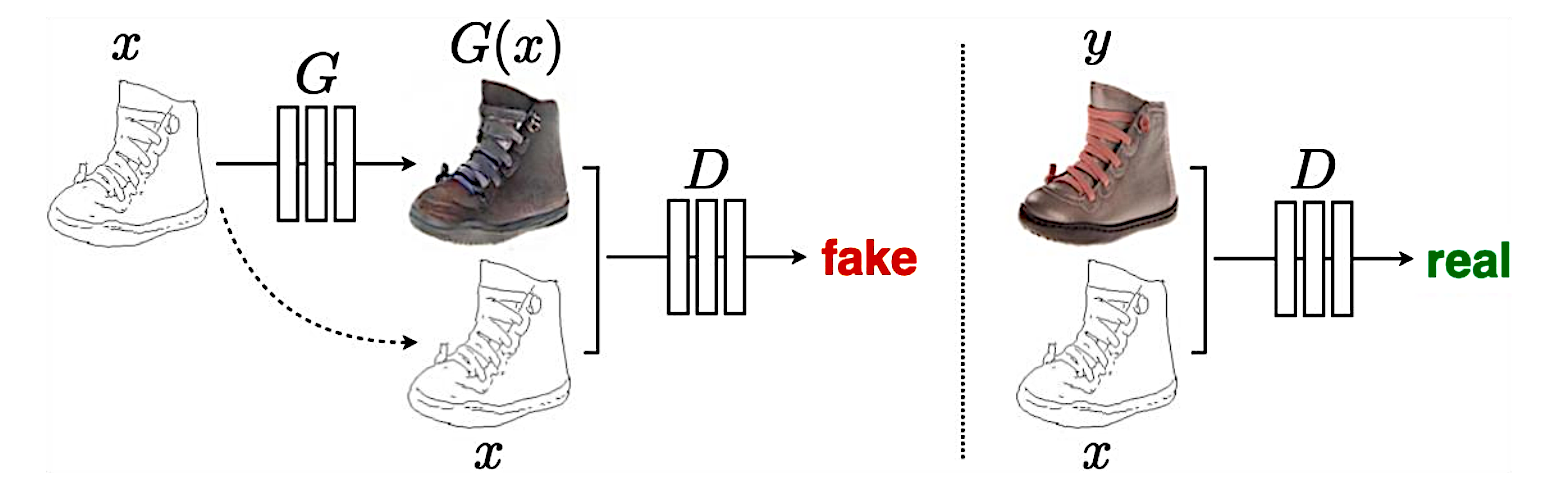
\includegraphics[width=0.7\linewidth]{img/conditional_GAN_edge_map}
	\caption{In conditional GANs both the Generator $G$ and the Discriminator $D$ input the edge map}
	\label{fig:conditionalganedgemap}
\end{figure}

\subsubsection{Conditional GANs}
Generator Architectures
\begin{figure}[H]
	\centering
	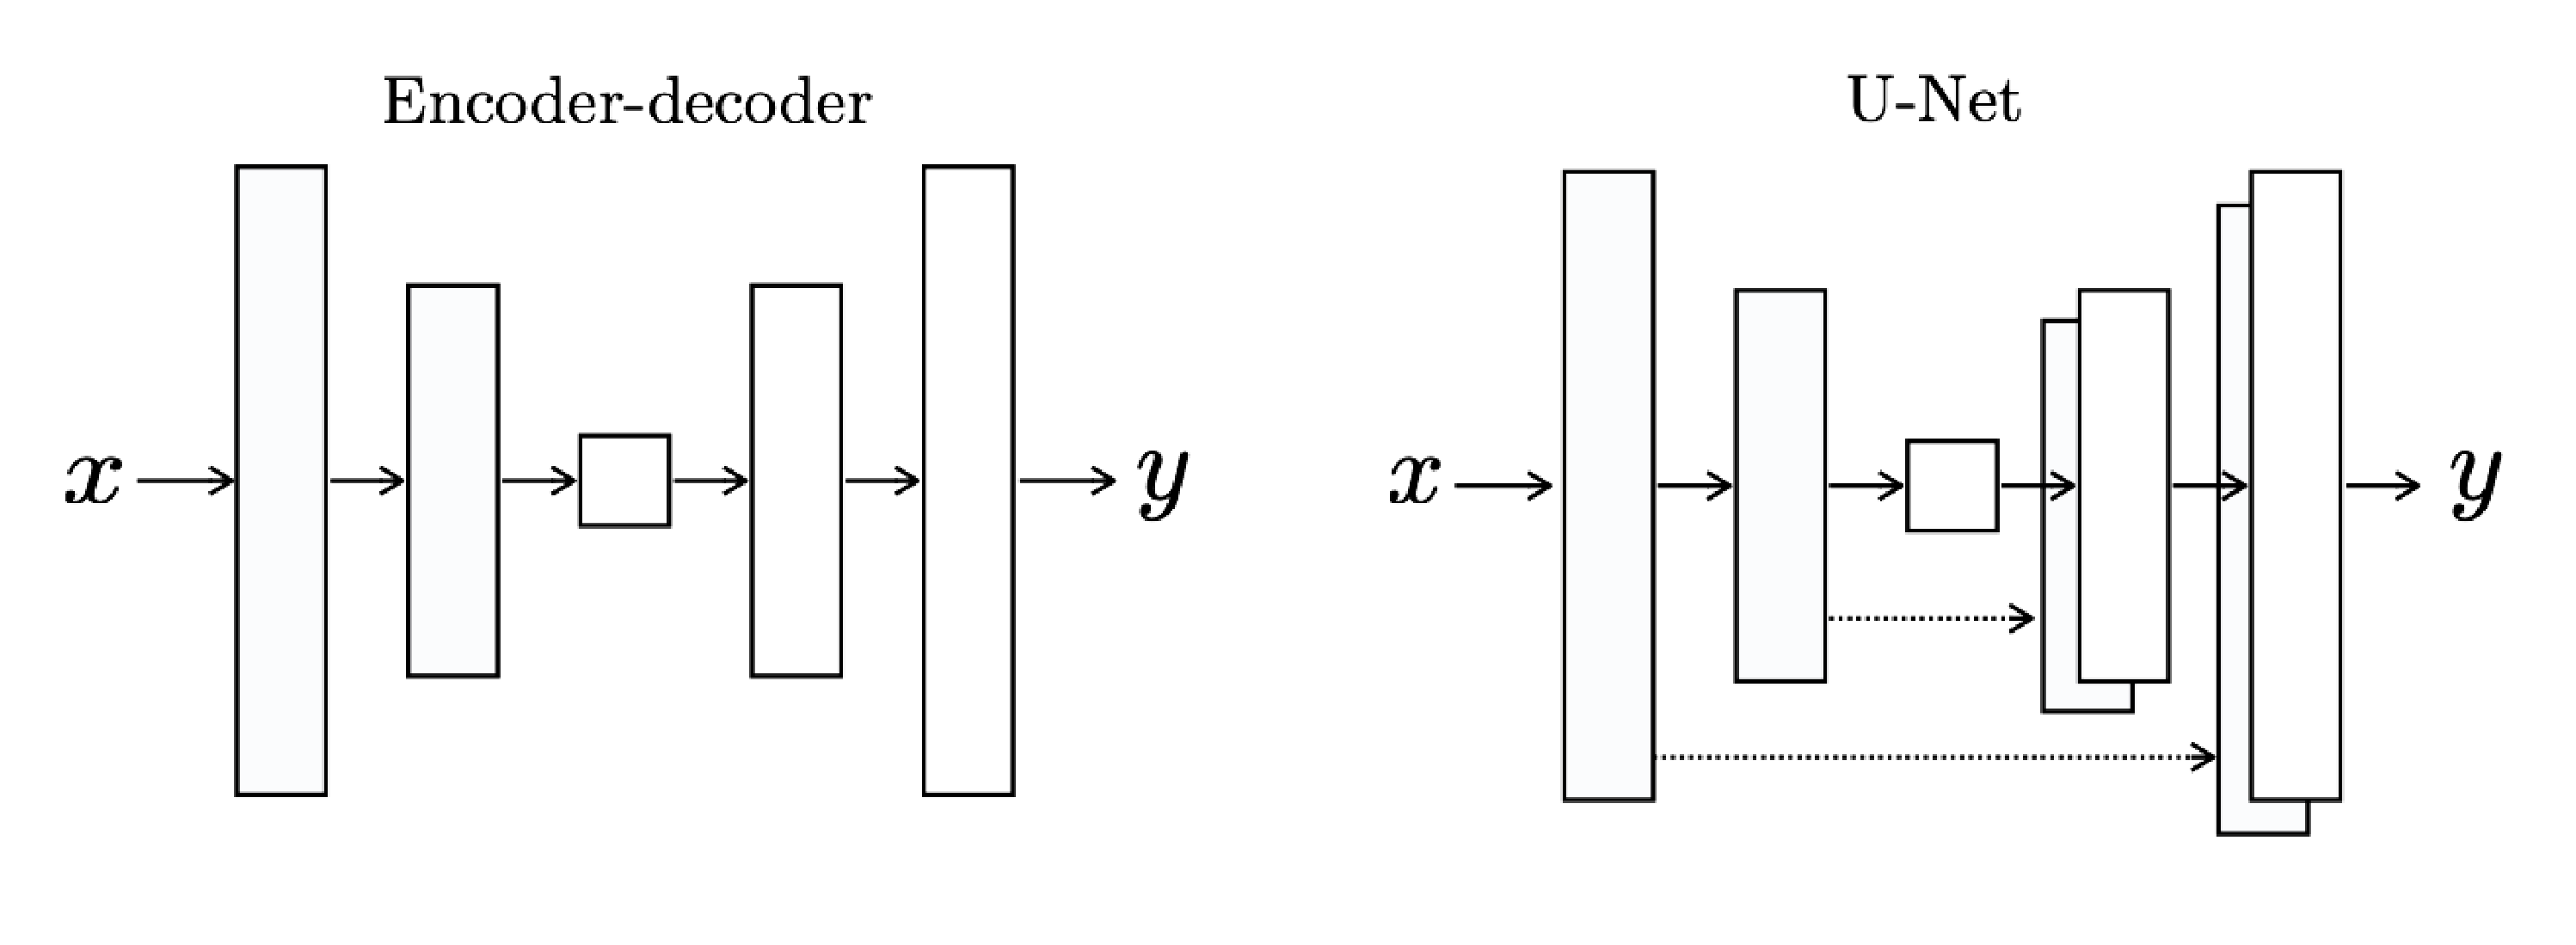
\includegraphics[width=0.7\linewidth]{img/conditional_GAN_generator_architectures}
	\caption{U-Net architectures with connections between the layers seem to work better}
	\label{fig:conditionalgangeneratorarchitectures}
\end{figure}

\subsection{Neural Texture Synthesis}
Given a low resolution texture image can a larger image be generated? For this there are two main approaches
\begin{itemize}[label=-]
	\item Replicate pixels and patches using a suitable algorithm
	\item Find a model of the texture and generate new textures from the model
\end{itemize}

\subsubsection{Texture Synthesis Using CNNs}
Pass image$x$ through the network, the activations from each layer are then the feature maps $F^l \in \R^{N\times M}$ for the texture.
Calculate the Gram matrix to compute correlations between feature maps (on the same layers)
\begin{equation*}
	G_{ij}^l = \sum_{k} F_{ik}^l F_{jk}^l
\end{equation*}
These Gram matrices describe the texture model.

\subsubsection{Generating Textures}
\begin{enumerate}[itemsep=0em]
	\item Start with noise image
	\item Use gradient descend to find another image that matches the Gram-matrix representation of the original image
	\item Optimize my minimizing the mean-squared distance between the matrices from the original and generated image
\end{enumerate}

\begin{center}
	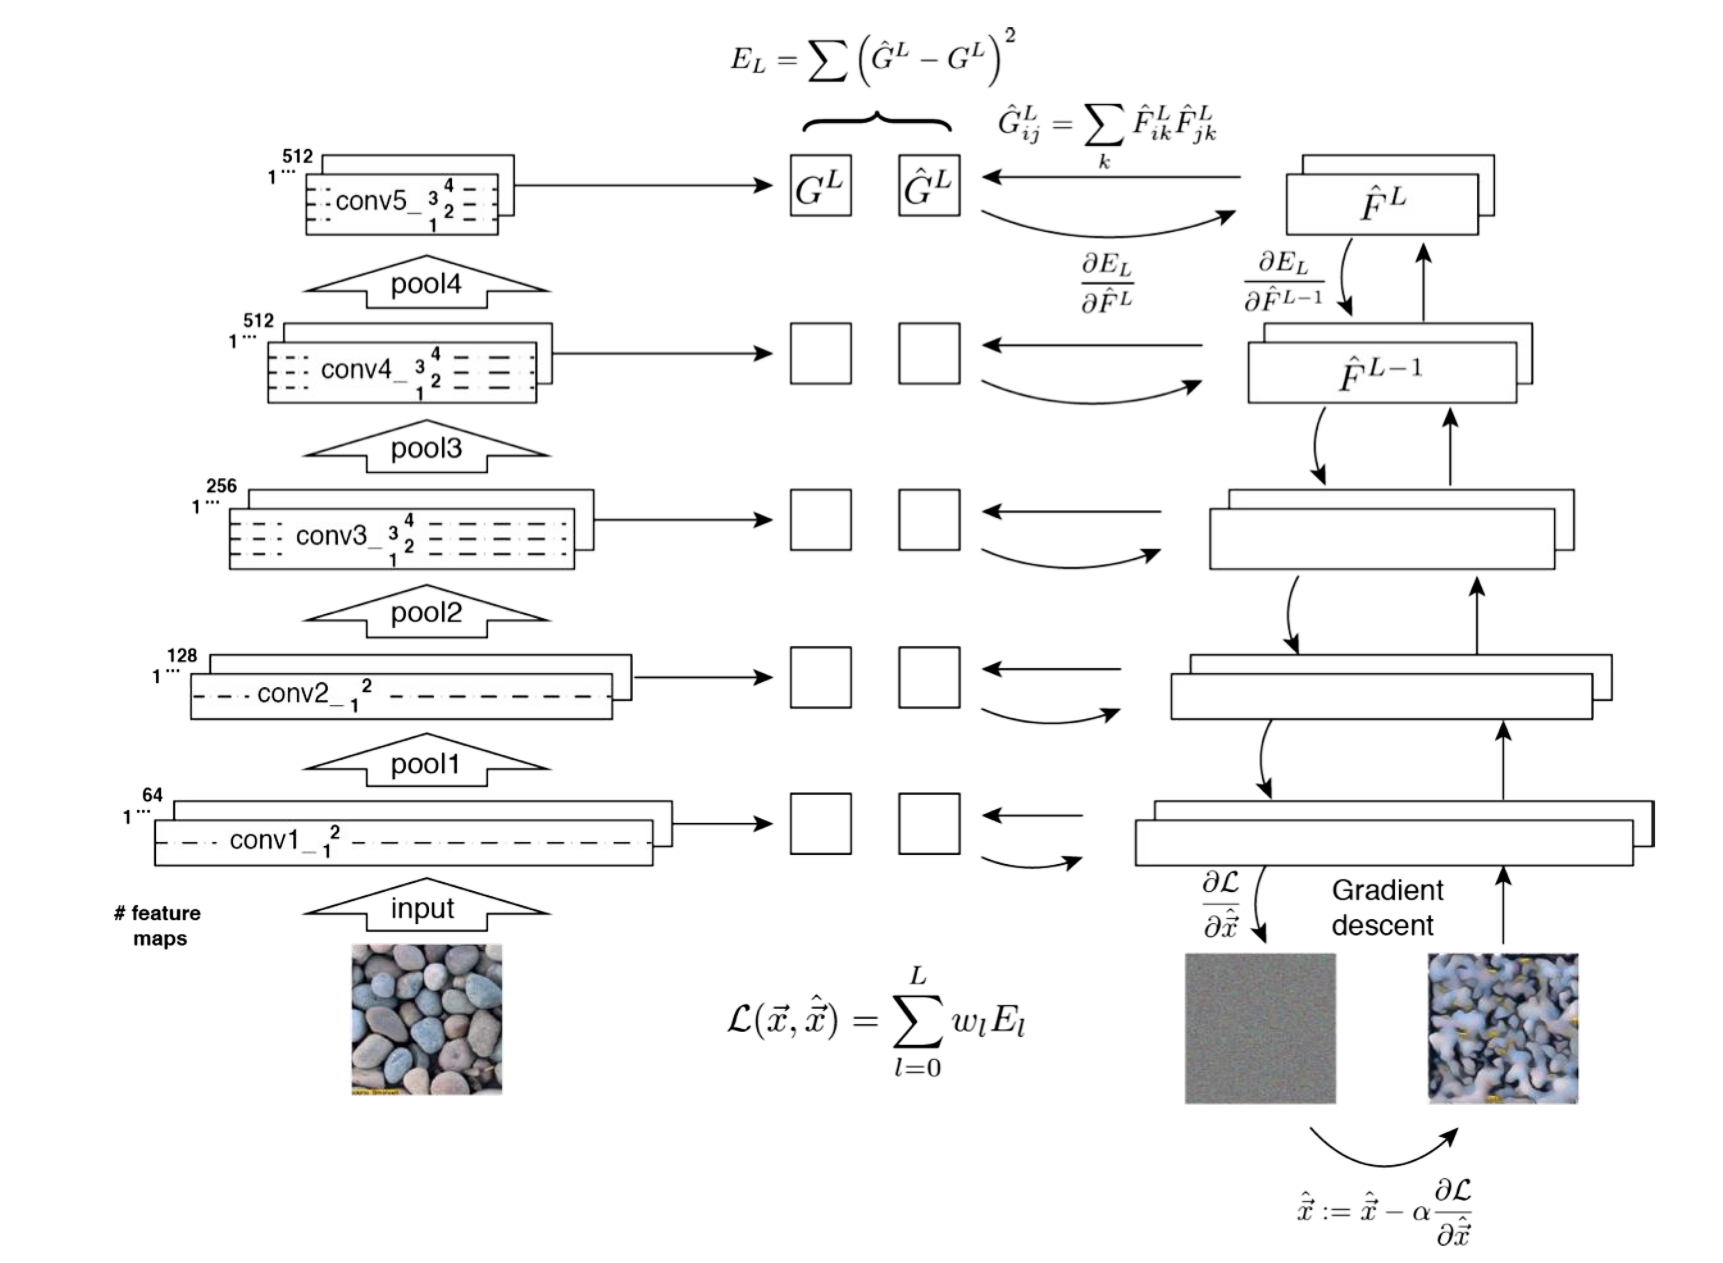
\includegraphics[width=0.8\linewidth]{img/conditional_GAN_texture_generation}
\end{center}

\subsection{Neural Style Transfer}
\begin{center}
	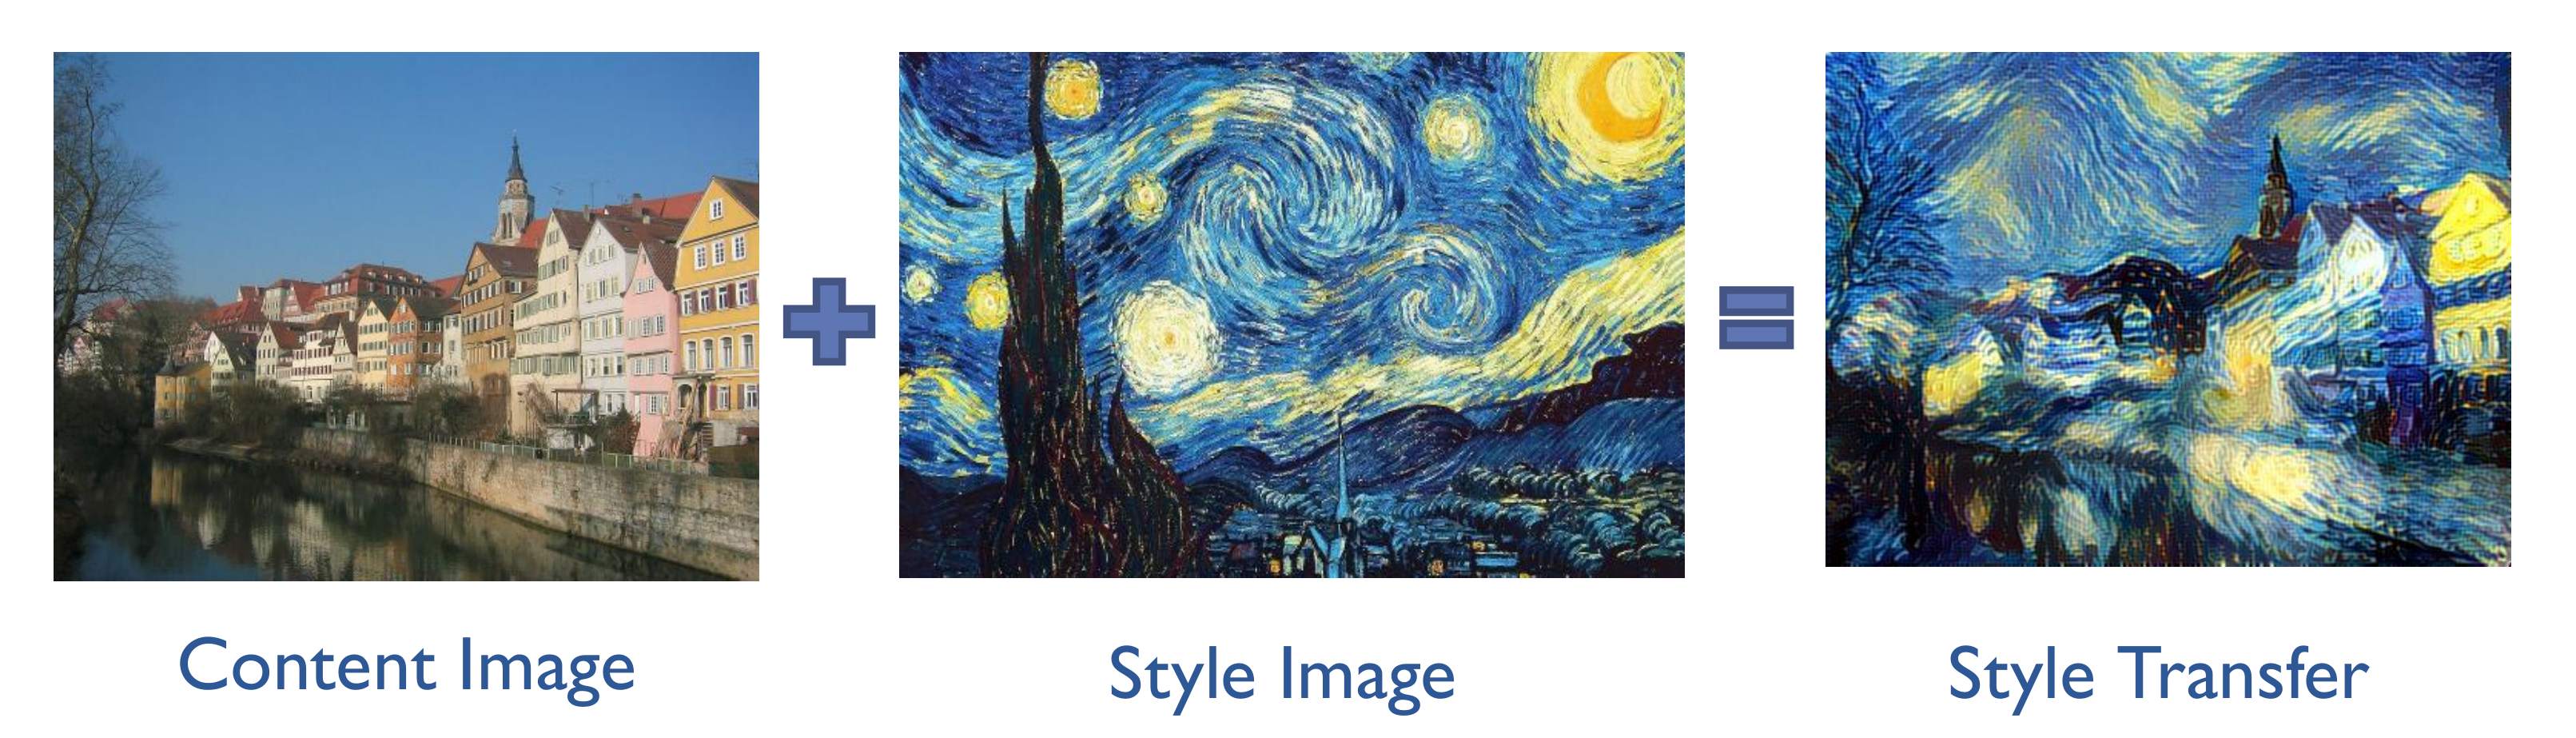
\includegraphics[width=0.7\linewidth]{img/conditional_GAN_style_transfer}
\end{center}

\subsubsection{Content Representation}
Each input image generates filter responses $F^l \in \R^{N\times M}$ at each layer.
Run gradient descend on noise images to find an image that generates the same response.
If $F^l \in \R^{N\times M}$ is the response from the original image and $P^l \in \R^{N\times M}$ the response from the generated image, the loss is
\begin{equation*}
	\L_{\text{content}}(\vec{p},\vec{x},l) = \frac{1}{2} \sum_{i,j} (F_{ij}^l - P_{ij}^l)^2
\end{equation*}
Later layers in the network define the content

\subsubsection{Style Representation}
Each input image generates filter responses $F^l \in \R^{N\times M}$ at each layer, calculate Gram matrices from the features.
If $A^l$ is the matrix from the original  image and $G^l$ the matrix from the generated image, the loss for one layer is
\begin{equation*}
	E_l = \frac{1}{4 N_l^2 M_l^2}\sum_{i,j}(G_{ij}^l - A_{ij}^l)^2
\end{equation*}
and including several layers
\begin{equation*}
	\L_{\text{style}}(\vec{a},\vec{x}) = \sum_{l=0}^{L}w_l E_l
\end{equation*}

\begin{center}
	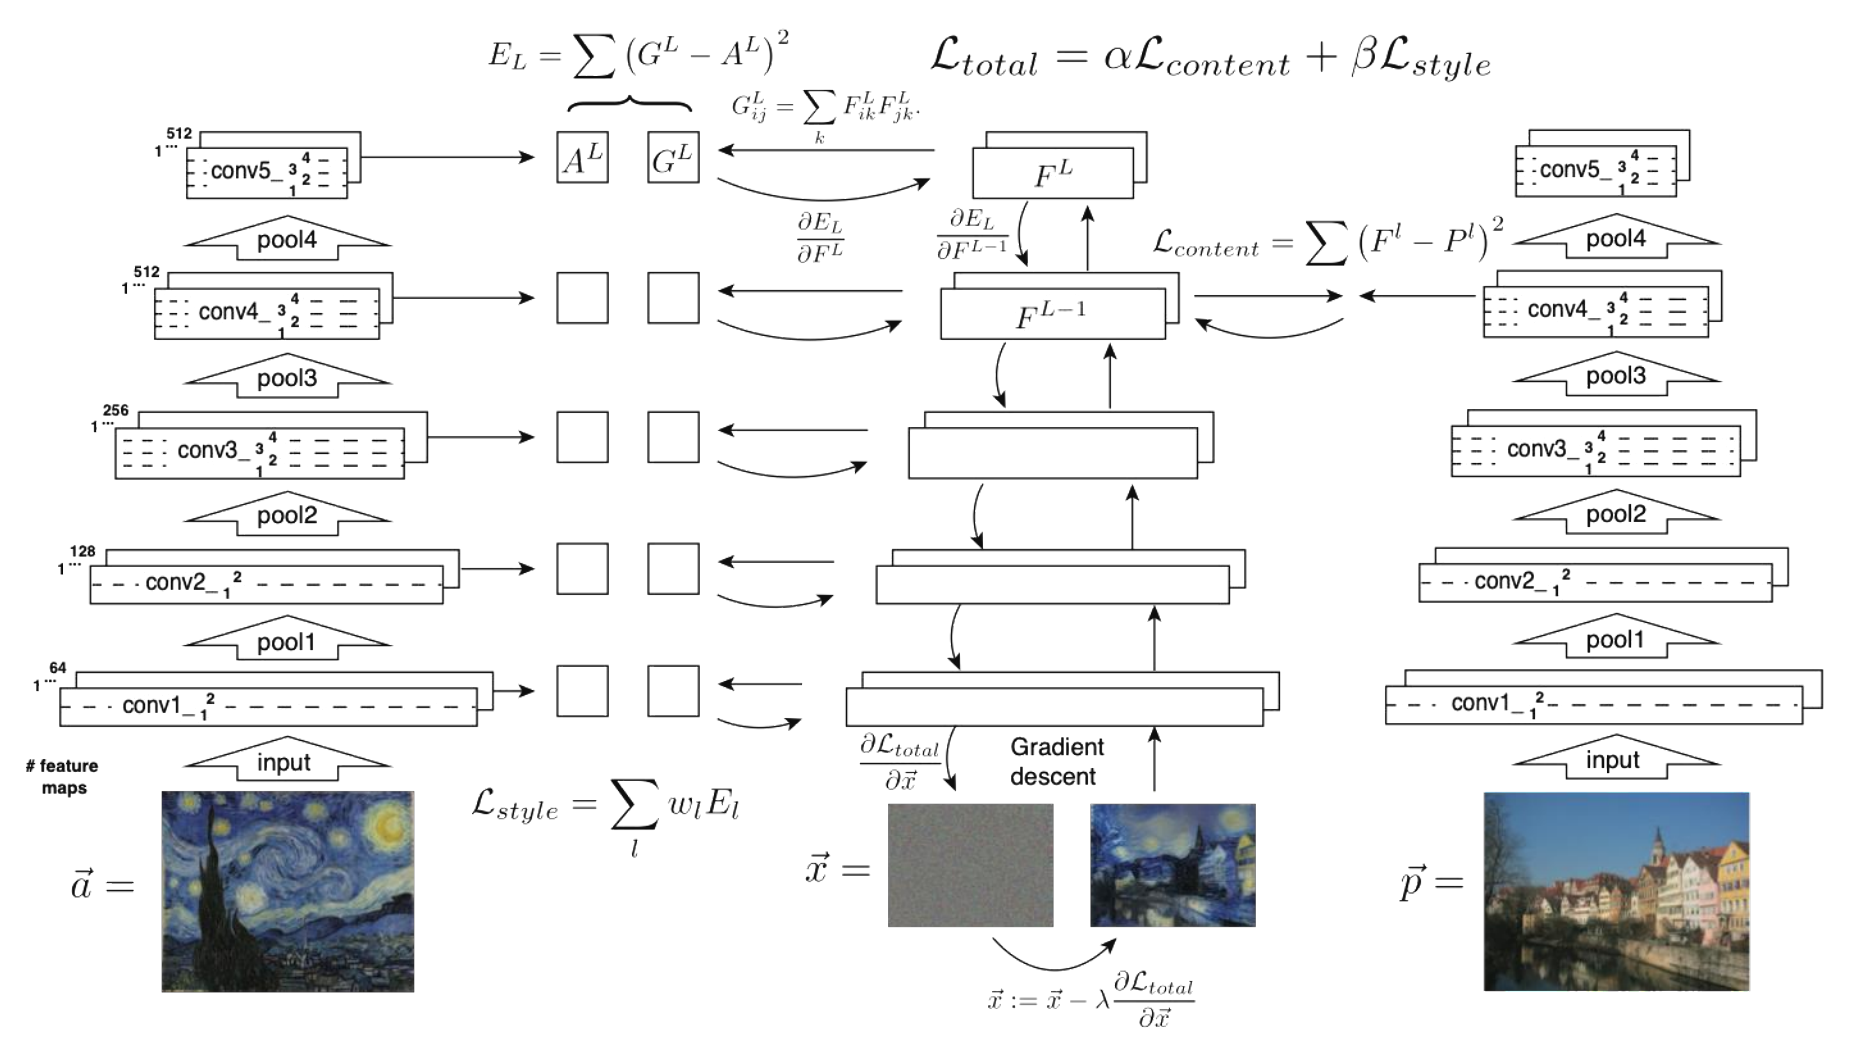
\includegraphics[width=0.8\linewidth]{img/conditional_GAN_style_representation.png}
\end{center}

\subsubsection{Fast Style Transfer}
The problem is that style transfer is slow as it requires many passes through VNN, the solution is to train a neural network to perform style transfer.
Train feedforward network for each style, use pretrained CNN with losses as before, and After training, stylize image with single forward pass.
\begin{center}
	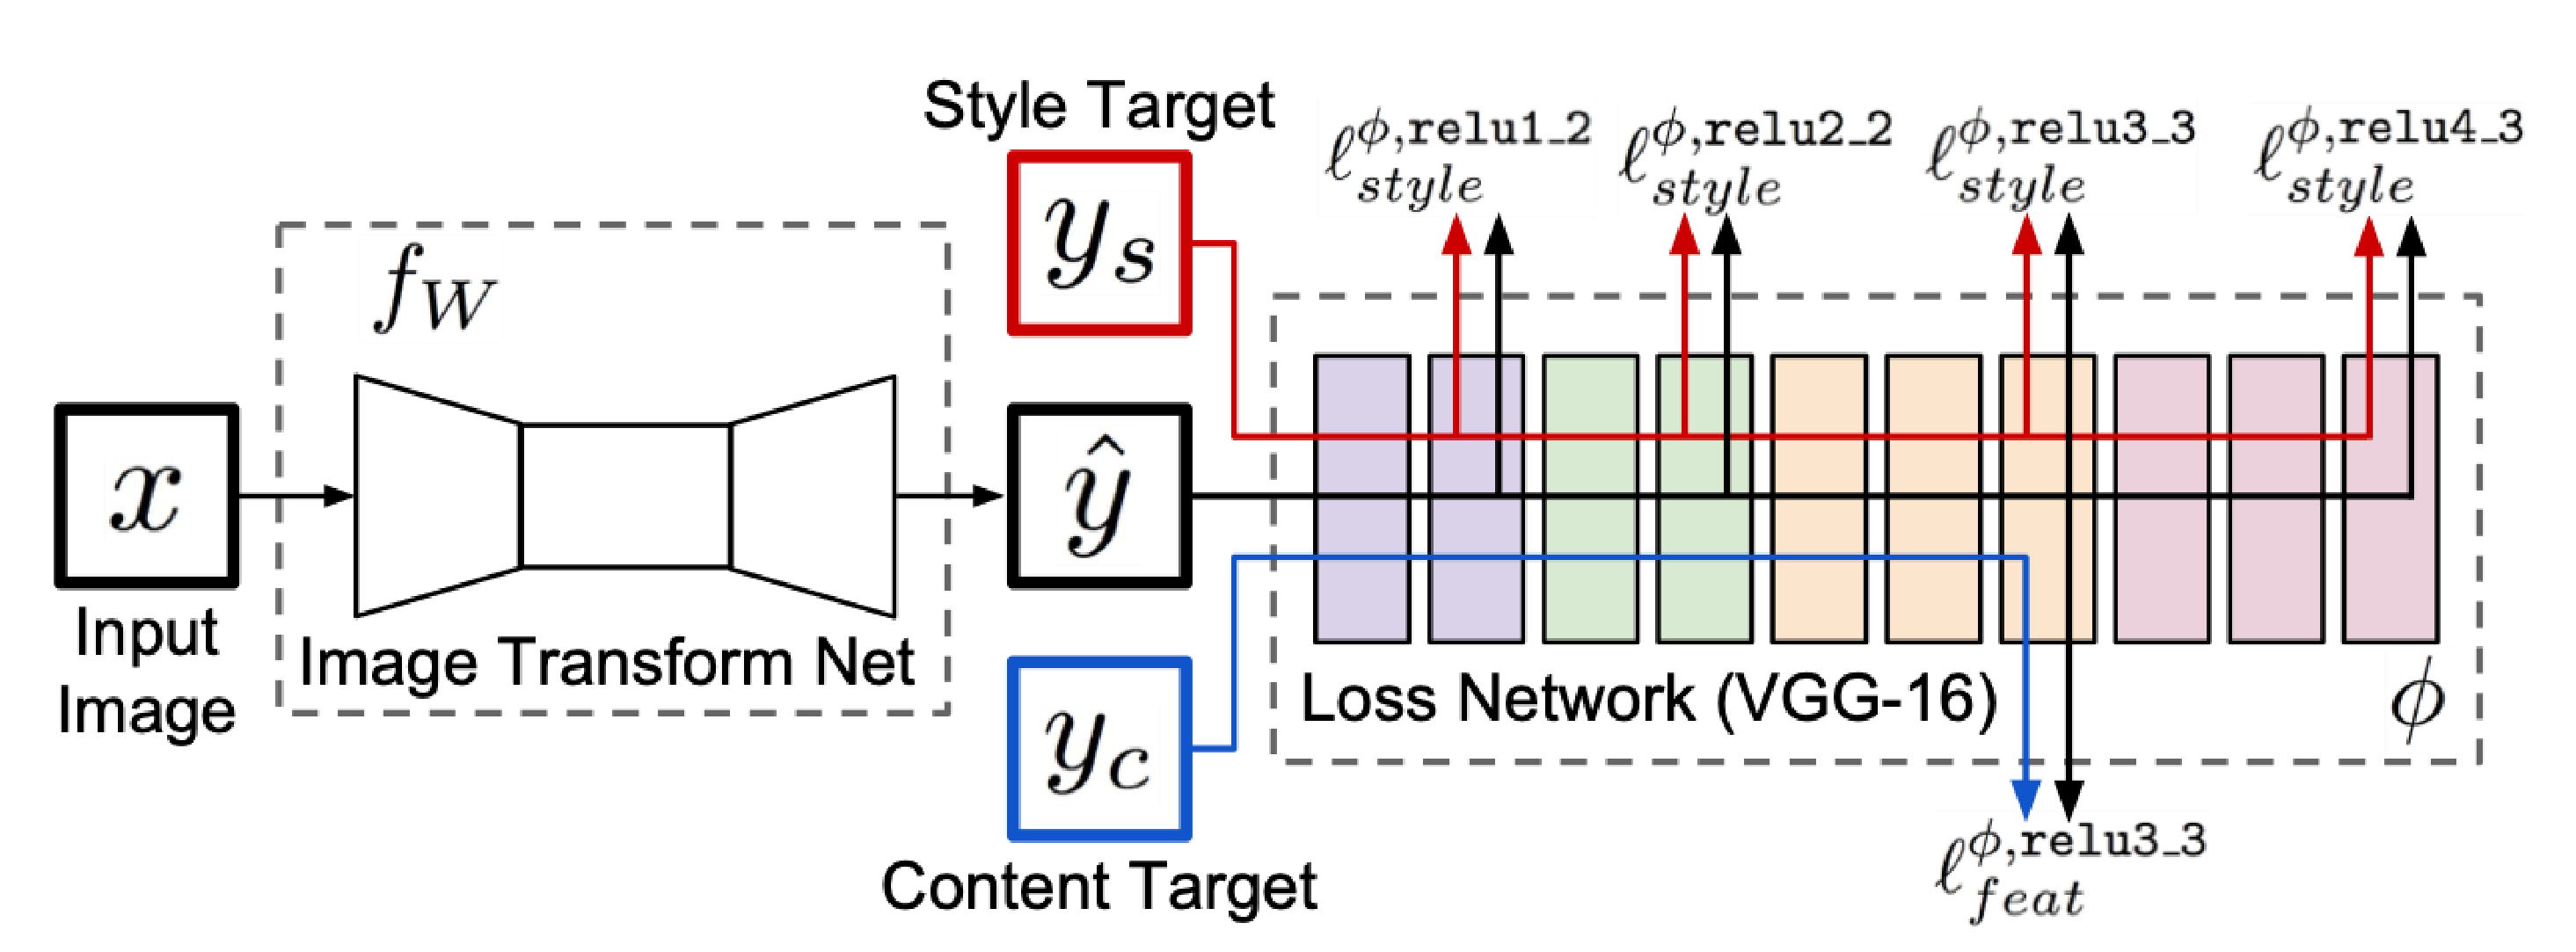
\includegraphics[width=0.7\linewidth]{img/fast_style_transfer}
\end{center}
